
\begin{ccHtmlOnly}
<center>
<img border="0" src="ball.gif" align="center">
</center>
\end{ccHtmlOnly} 

\begin{ccTexOnly}
\begin{center}
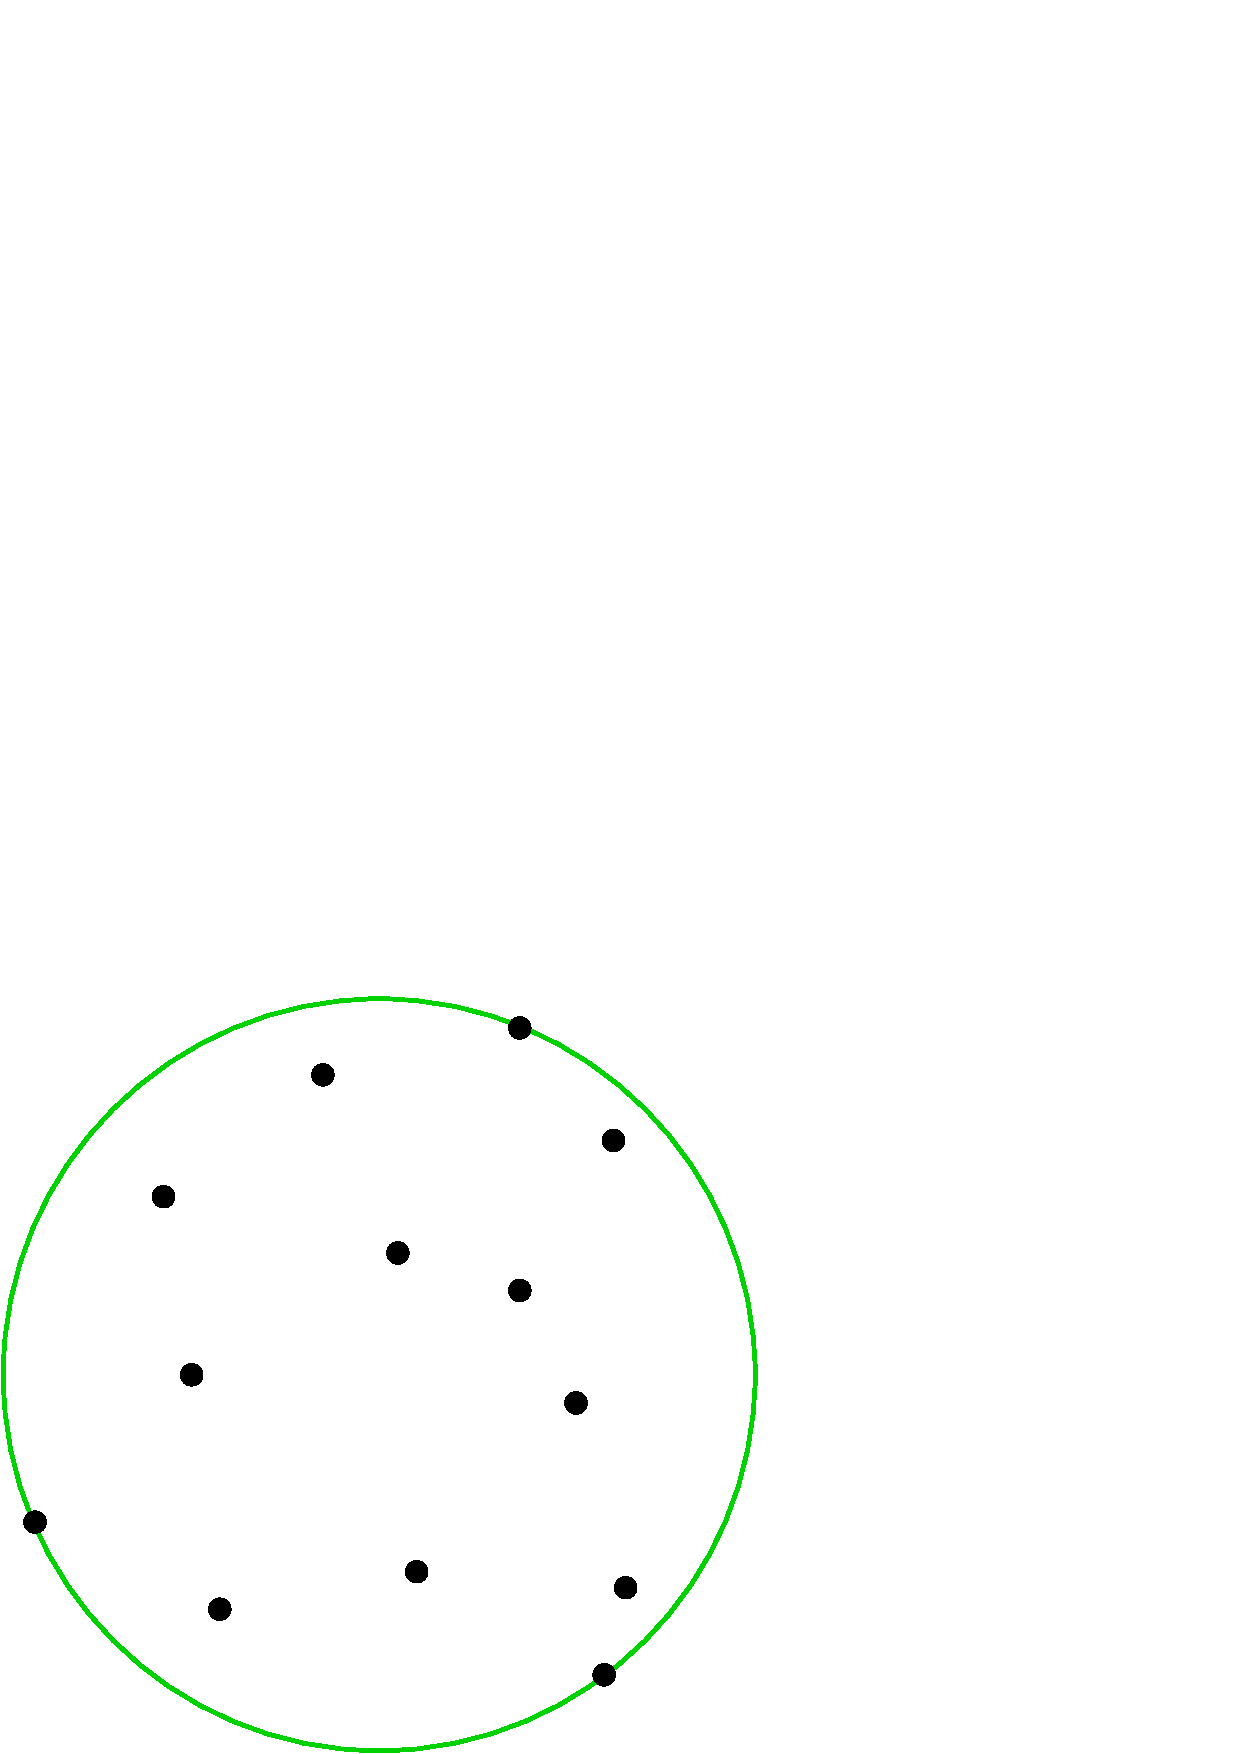
\includegraphics[width=4cm]{Bounding_volumes/ball}
%%\leavevmode\epsfxsize8cm\epsffile{ball.eps}
\end{center}
\end{ccTexOnly}


This chapter describes algorithms which for a given point set compute
the ``best'' circumscribing  object from a specific
class. If the class consists of all spheres in $d$-dimensional
Euclidean space and ``best'' is defined as having smallest radius,
then we obtain the smallest enclosing sphere problem already mentioned
above.

In the following example a smallest enclosing circle
(\ccc{CGAL::Min_circle_2<Traits>}) is constructed from points 
on a line and written to standard output. The example
shows that it is advisable to switch on random shuffling 
in order to deal with a `bad' order of the input points. 
%%The default traits class is used here.

\ccIncludeExampleCode{Min_circle_2/min_circle_2.cpp}

Other classes for which we provide solutions are ellipses
(\ccc{CGAL::Min_ellipse_2<Traits>}), rectangles
(\ccc{CGAL::min_rectangle_2}), parallelograms
(\ccc{CGAL::min_parallelogram_2}) and strips (\ccc{CGAL::min_strip_2})
in the plane, with appropriate optimality criteria. For arbitrary
dimensions we provide smallest enclosing spheres for points
(\ccc{CGAL::Min_sphere_d<Traits>}) and spheres for spheres
(\ccc{CGAL::Min_sphere_of_spheres_d<Traits>}), smallest enclosing
annuli (\ccc{CGAL::Min_annulus_d<Traits>}), and approximate
minimum-volume enclosing ellipsoid with user-specified
approximation ratio (\ccc{CGAL::Approximate_min_ellipsoid_d<Traits>}).

\begin{ccHtmlOnly}
<center>
<img border="0" src="annulus.gif" align="center">
</center>
\end{ccHtmlOnly} 

\begin{ccTexOnly}
\begin{center}
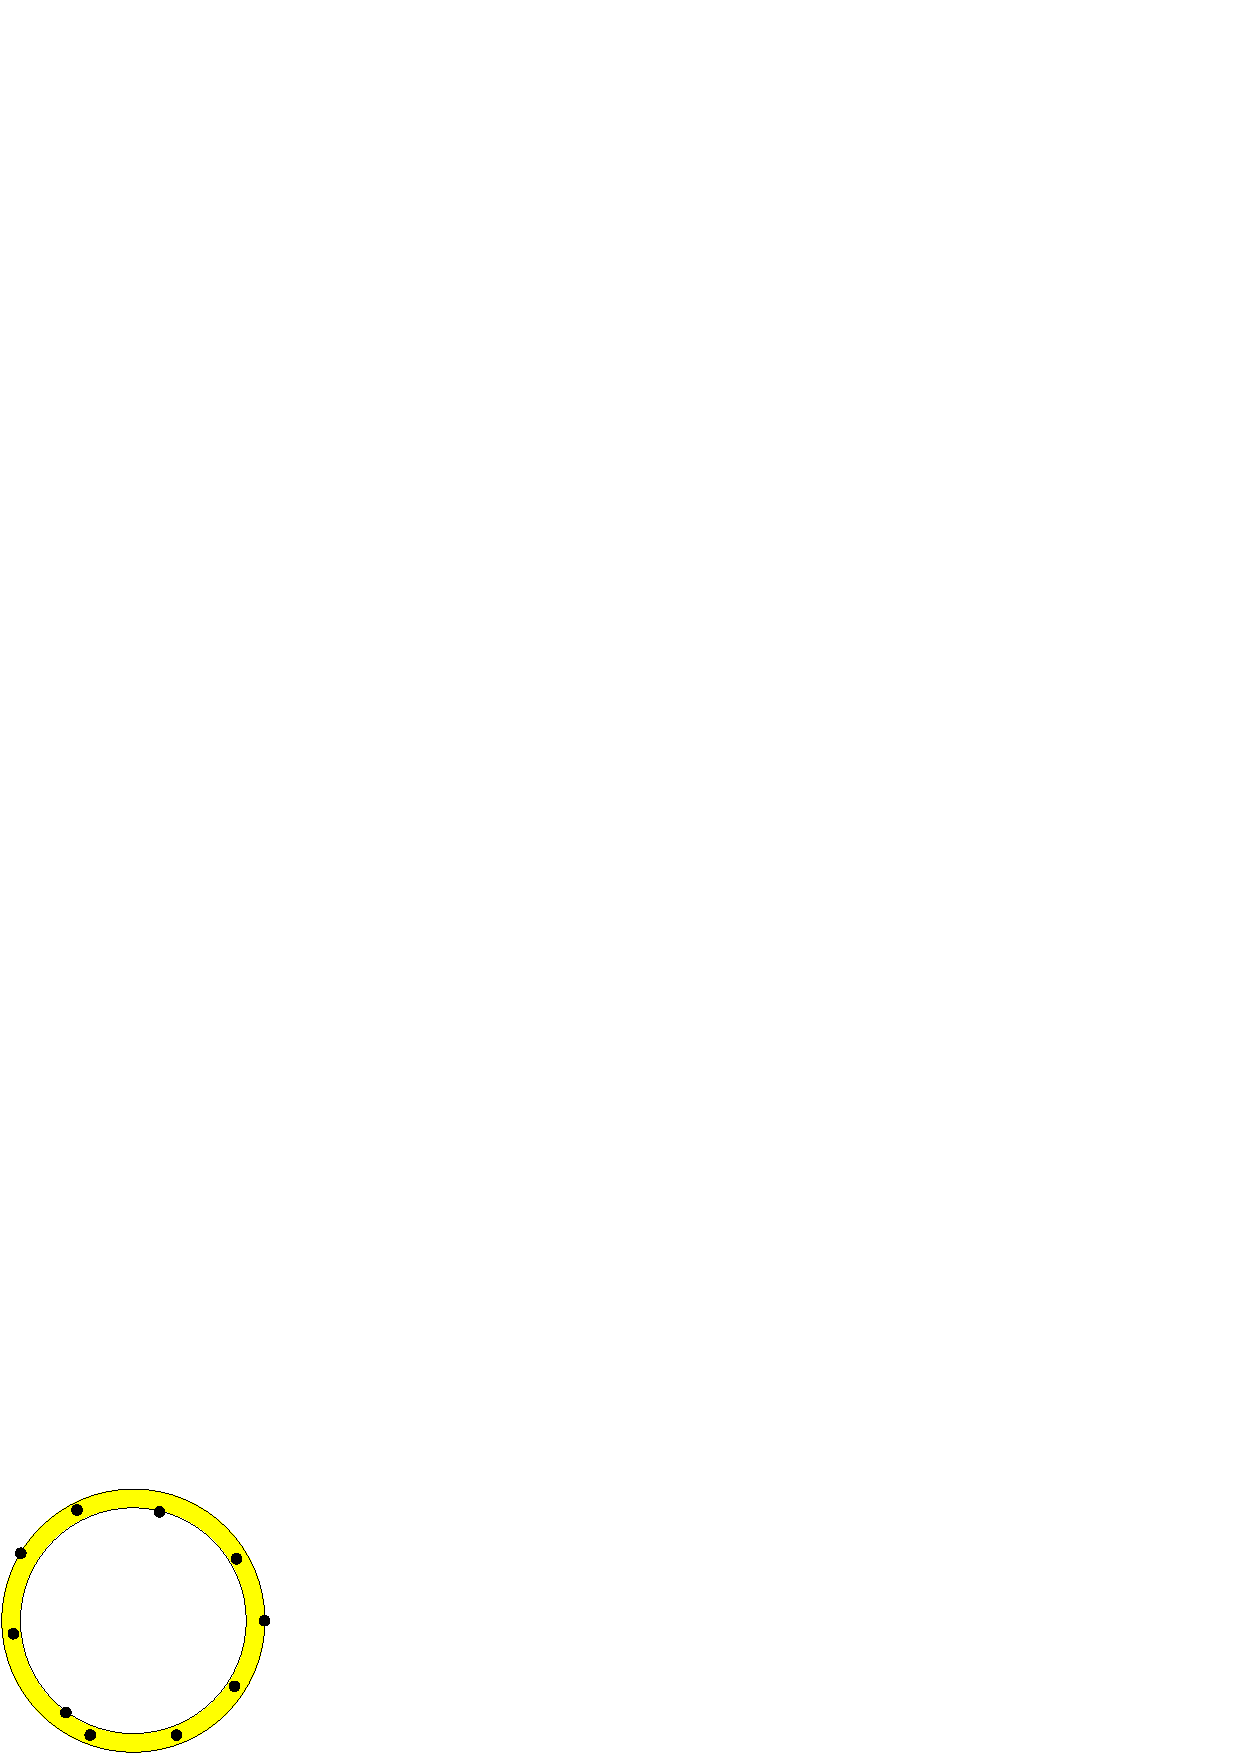
\includegraphics[width=4cm]{Bounding_volumes/annulus}
%%\leavevmode\epsfxsize8cm\epsffile{annulus.eps}
\end{center}
\end{ccTexOnly}

Bounding volumes can be used to obtain simple approximations of
complicated objects. For example, consider the problem of deciding
whether two moving polygons currently intersect. An obvious solution
is to discretize time and perform a full intersection test for any
time step. If the polygons are far apart most of the time, this is
unnecessary. Instead, simple bounding volumes (for examples, circles)
are computed for both polygons at their initial positions. At
subsequent time steps, an intersection test between the moving
bounding circles replaces the actual intersection test; only if the
circles do intersect, the expensive intersection test between the
polygons is performed. In practice, bounding volume hierarchies are
often used on top of simple bounding volumes to approximate
complicated objects more accurately.


Bounding volumes are also frequently applied to extract
geometric properties of objects. For example, the smallest enclosing
annulus of a point set can be used to test whether a set of points is
approximately cospherical. Here, the width of the annulus (or its
area, or still another criterion that we use) is a good measure for
this property. The largest area triangle is for example used in
heuristics for matching archaeological aerial photographs. Largest
perimeter triangles are used in scoring cross country soaring flights,
where the goal is basically to fly as far as possible, but still
return to the departure airfield. To score simply based on the total
distance flown is not a good measure, since circling in thermals
allows to increase it easily.

Bounding volumes also define geometric ``center points'' of objects.
For example, if two objects are to be matched (approximately), one
approch is to first apply the translation that maps the centers of
their smallest enclosing spheres onto each other.  Simpler centers are
possible, of course (center of gravity, center of bounding box), but
more advanced bounding volumes might give better results in some
cases. It can also make sense to consider several center points
instead of just one. For example, we provide algorithms to cover a
planar point set with between two and four minimal boxes
(\ccc{CGAL::rectangular_p_center_2}). Below is an example covering with
three boxes; the center points are shown in red.

\begin{ccHtmlOnly}
<center>
<img border="0" src="pcenter.gif" align="center">
</center>
\end{ccHtmlOnly} 

\begin{ccTexOnly}
\begin{center}
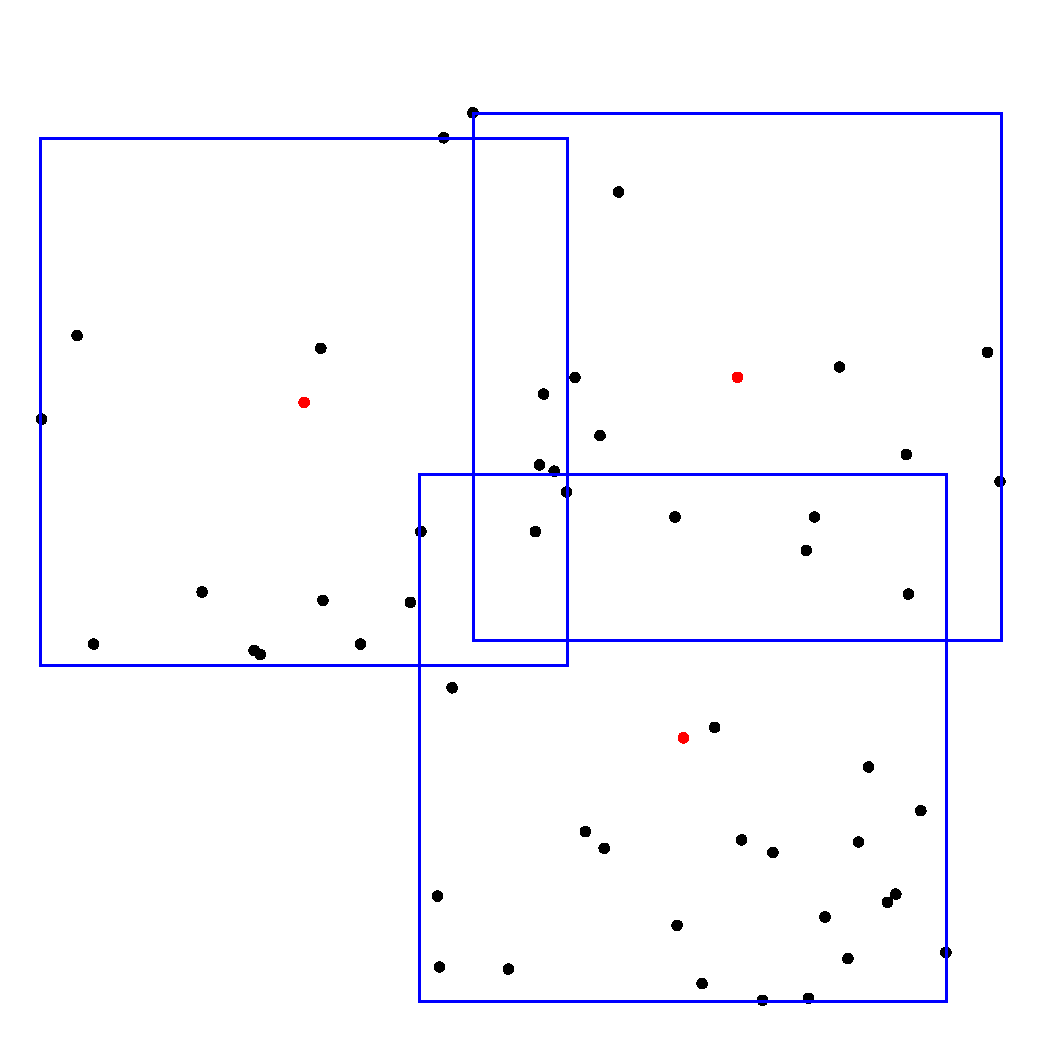
\includegraphics[width=5cm]{Bounding_volumes/pcenter}

\end{center}
\end{ccTexOnly}

%To avoid later disappointment: one very nice class of bounding
%volumes, namely ellipsoids in three- and higherdimensional space, is
%currently not supported by \cgal. The reason is that the algebraic
%complexity of this problem is still beyond the level which would allow
%us to come up with a solution that satisfies the \cgal\ standards. We
%are working on a solution for 3-space, though.


%% ===== EOF ===================================================================



